\chapter{An improved framework for downscaling cloud properties from large-scale models}\label{sgi_chapter}
The previous chapter identified errors in simulated satellite cloud diagnostics that arise in using unrealistic cloud overlap assumptions and homogeneous condensate. In this chapter, an improved subcolumn generator is presented, building on the work of previous investigators, to reduce those errors and enable more consistent and robust comparisons of modeled and satellite-retrieved cloud statistics. 

The improved subcolumn generator described here uses a scheme developed by \cite{raisanen_et_al_2004} to generate subcolumn cloud condensate that both follows a more realistic overlap assumption and allows for generating subcolumn condensate with horizontal variability. This scheme has been extended here to apply to precipitation as well, and condensate variability and overlap parameters are also parameterized using a combination of high-resolution global model output from the SP-CAM and observations from the CloudSat and CALIPSO [?].

\section{Generating stochastic subcolumns of cloud and precipitation condensate}
\label{subgrid2_generator_section}
\cite{raisanen_et_al_2004} (hereafter R04) introduce a stochastic subcolumn generator that can handle both horizontally variable condensate and generalized cloud overlap. In the R04 scheme, subcolumn cloud occurrence is first determined by assuming that cloud overlap between adjacent layers is a linear combination of maximum and random overlap, such that the combined cloud fraction between two layers $k_1, k_2$ is
\begin{gather}
c_{k_1, k_2}^{\rm gen} = \alpha_{k_1, k_2} c_{k_1, k_2}^{\rm max} + (1 - \alpha_{k_1, k_2})
c_{k_1, k_2}^{\rm ran}
    \label{generalized_overlap_equation}
\end{gather}
where $c_{k_1, k_2}^{\rm gen}$ is the actual combined (vertically projected) cloud fraction that would result from generalized overlap, $c_{k_1, k_2}^{\rm max}$ is the cloud fraction that would result if the layers were maximally overlapped, $c_{k_1, k_2}^{\rm ran}$ is the cloud fraction that would result if the layers were randomly overlapped, and $\alpha_{k_1, k_2}$ is the ``overlap parameter'' that specifies the weighting between maximum and random overlap. The theoretical combined cloud fractions $c^{\rm max}_{k_1, k_2}$ and $c^{\rm ran}_{k_1, k_2}$ are defined as
\begin{gather}
    c^{\rm max}_{k_1, k_2} = \max(c_{k_1}, c_{k_2}) \\
    c^{\rm ran}_{k_1, k_2} = c_{k_1} + c_{k_2} - c_{k_1} c_{k_2}
\end{gather}

Given $\alpha_{k_1, k_2}$ and the cloud fraction $c_{k}$ at each layer, R04 describe a straightforward algorithm to stochastically generate a binary subcolumn clear/cloudy flag that obeys the above overlap relationship by stepping down from the top of the atmospheric column and considering only adjacent layer pairs. First, for each subcolum $i$ and at each level $k$, three random numbers on the interval $[0, 1)$ are drawn, denoted $R1_{i, k}$, $R2_{i, k}$, and $R3_{i, k}$. A variable $x_{i, k}$ is then generated as follows. At level $k = 1$ (TOA), $x_{i, 1}$ is set to $x_{i, 1} = R1_{i, 1}$. Levels $k$ and columns $i$ are then iterated over from $k = 2, \ldots, n_{\rm lev}$ and $i = 2, \ldots, n_{\rm col}$, and at each level, $x_{i, k}$ is determined by
\begin{align}
    x_{i, k} = \begin{cases} 
        x_{i, k-1}, ~ & R2_{i, k} \le \alpha_{k-1, k} \\
        R3_{i, k}, ~ & R2_{i, k} > \alpha_{k-1, k}
    \end{cases}
\end{align}
From this, the binary cloudy/clear flag $b^{\rm cloud}_{i, k}$ is determined from the value of $x_{i, k}$ and the cloud fraction $c_{k}$ at level $k$ by
\begin{align}
    b^{\rm cloud}_{i, k} = \begin{cases}
        1, ~ & x_{i, k} > 1 - c_{k}, \\
        0, ~ & x_{i, k} \le 1 - c_{k}
    \end{cases}
\end{align}

Once the binary subcolumn cloud occurrence subcolumns are created, cloud condensate is assigned to the cloudy columns by drawing from an assumed probability distribution for condensate. Condensate values are drawn such that the generated columns obey a specified rank correlation $\rho_{k_1, k_2}$ for condensate amount between adjacent layers, where $\rho_{k_1, k_2}$ is the Pearson Product-Moment Correlation coefficient of the ranks $r_{k_1}$ and $r_{k_2}$ of condensate at laevels $k_1$ and $k_2$, such that
\begin{gather}
    \rho_{k_1, k_2} = \frac{
        {\rm cov}(r_{k_1}, r_{k_2})
    }{
        \sigma_{r_{k_1}} \sigma_{r_{k_2}}
    } = \frac{
        \sum_{i=1}^{n_{\rm col}} (r_{i, k_1} - \overline{r_{k_1}})(r_{i, k_2} - \overline{r_{k_2}})
    }{
        \sqrt{\sum_{i=1}^{n_{\rm col}} (r_{i, k_1} - \overline{r_{k_1}})^2}
        \sqrt{\sum_{i=1}^{n_{\rm col}} (r_{i, k_2} - \overline{r_{k_2}})^2}
    }
    \label{rankcorr_equation}
\end{gather}
This is done by first generating a variable $y_{i, k}$ at each subcolumn $i$ and level $k$ analogous to the variable $x_{i, k}$ used to determine the binary occurrence flag. Again, three sets of random numbers $R4_{i, k}$, $R5_{i, k}$, and $R6_{i, k}$ on the interval $[0, 1)$ are drawn at each subcolumn $i$ and level $k$. The top ($k = 1$) layer is set to $y_{i, 1} = R4_{i, 1}$. For each subsequent level,
\begin{align}
    y_{i, k} = \begin{cases}
        y_{i, k-1}, ~ & R5_{i, k} \le \rho_{k-1, k} \\
        R6_{i, k},  ~ & R5_{i, k} > \rho_{k-1, k}
    \end{cases}
\end{align}
With this, and an assumed probability distribution for condensate amount with probability density function $p_k(q)$ at level $k$, where $q$ is the condensate amount (specified as a mass mixing ratio), the condensate amount $q_{i, k}$ at each level is determined by finding $q_{i, k}$ such that
\begin{align}
    y_{i, k} = \int_0^{q_{i, k}} p_{k}(q') ~dq'
\end{align}

The problem of generating stochastic subcolumns of cloud condensate with generalized occurrence overlap and heterogeneous condensate distributions then reduces to specifying the parameters $\alpha_{k_1, k_2}$ and $\rho_{k_1, k_2}$ for each pair of \emph{adjacent} layers within a gridbox, and specifying an appropriate probability distribution from which to sample condensate amount. The cloud occurrence overlap is often fit to an inverse exponential function of the separation  between layers, such that
\begin{gather}
    \alpha_{k_1, k_2} = \exp\left(-\frac{z_{k_1} - z_{k_2}}{z_0}\right)
    \label{alpha_exponential_equation}
\end{gather}
where $z_{k_1}$ and $z_{k_2}$ are the heights of layers $k_1$ and $k_2$, and $z_0$ is the ``decorrelation length'' for cloud overlap that specifies how quickly
the vertical correlation in cloud occurrence decays from maximal to random
\citep{hogan_and_illingworth_2000, mace_and_benson-troth_2002,
raisanen_et_al_2004, pincus_et_al_2005, barker_2008}. \cite{raisanen_et_al_2004} and \cite{pincus_et_al_2005} further
suggest that the same exponential relationship can describe the rank
correlation of condensate, but in general using a separate decorrelation length.
These studies have suggested decorrelation lengths for cloud occurrence overlap between 1.5 and 2.5 km, and somewhat smaller decorrelation lengths for condensate rank correlation. Overlap and decorrelation lengths will be parameterized in the following section for use with the SP-CAM output used in this study. 

The R04 subcolumn generator was designed specifically for generating stochastic subcolumns of \emph{cloud} condensate. However, as shown in the previous chapter, the treatment of subcolumn precipitation is critical to obtaining reasonable simulations of radar reflectivity factor from large scale model output. The R04 generator is extended here to also generate stochastic subcolumns of \emph{precipitation} condensate with horizontally heterogeneous condensate amount. %The following describes the extension of the \cite{raisanen_et_al_2004} subcolumn generator to also generate stochastic subcolumns of \emph{precipitation} condensate. 

%Since only adjacent layers are considered in the \cite{raisanen_et_al_2004} subcolumn generator, the appropriate values for $z_0$ will in general be dependent on the vertical resolution, since the ``separation distance'' considered is simply the separation between vertical level midpoints [elaborate on this].
%[Question: does the combination of generalized overlap with PREC\_SCOPS, with the precipitation adjustment produce the right precipitation overlap and the right cross-correlation between cloud and precip? Or do we need a more sophisticated treatment?] 

The simplest way to extend this subcolumn scheme to also handle precipitation is to first generate the binary cloud flag $b^{\rm cloud}_{i, k}$ using the subcolumn generator described above. The subcolumn precipitation flag $b^{\rm precip}_{i, k}$ is then generated using the PREC\_SCOPS routine from COSP, with the precipitation adjustment described in the previous chapter to constrain the number of precipitating subcolumn elements by the precipitation fraction from the model. The subcolumn precipitation condensate amount is then prescribed in a similar manner to the subcolumn cloud condensate amount but with a separate rank correlation for precipitation, and a separate assumed probability distribution. 

As an alternative to this, the precipitation flag $b^{\rm precip}_{i, k}$ can be generated in a similar manner to the cloudy flag $b^{\rm cloud}_{i, k}$, but with $\alpha_{i, k}$ replaced with the overlap for \emph{precipitation} $\alpha^{\rm precip}_{i, k}$. The advantage of this second formulation is that the overlap of precipitation would be precisely reproduced, and the dependence on the precipitation fraction is built in. However, this does not preserve the cross-correlation between cloud and precipitation occurrence. [!!! this paragraph needs to be re-worked !!!]

The above presents a complete subcolumn generator that can produce subcolumns with generalized cloud occurrence overlap, prescribed precipitation occurrence fraction, and horizontally heterogeneous cloud and precipiation condensate, given the occurrence overlap decorrelation length for cloud, the decorrelation lengths for condensate amount rank correlation, and assumed probability distributions for cloud and precipitation condensate amounts. The following sections describe parameterizing these quantities for use in the sensitivity study to follow.

\section{Parameterizing occurrence overlap and rank correlation from SP-CAM}
\label{subgrid2_overlap_section}
In this chapter, occurrence overlap and rank correlation are derived from the same SP-CAM model output used in the previous chapter to evaluate sensitivities in COSP diagnostics to overlap. With the high-resolution model output provided by the SP-CAM, the occurrence overlap can be directly calculated following \cite{pincus_et_al_2005} for each gridbox from the subcolumn condensate by solving Equation \ref{generalized_overlap_equation} for $\alpha_{k_1, k_2}$ and assuming that the ``true'' combined cloud fraction between layers $k_1$ and $k_2$ can be described by generalized overlap, so that $c^{\rm true}_{k_1, k_2} = c^{\rm gen}_{k_1, k_2}$. This yields for the overlap parameter $\alpha$
\begin{gather}
    \alpha_{k_1, k_2} = \frac{
        c^{\rm true}_{k_1, k_2} - c^{\rm ran}_{k_1, k_2}
    }{
        c^{\rm max}_{k_1, k_2} - c^{\rm ran}_{k_1, k_2}
    }
    \label{alpha_equation}
\end{gather}
For each gridbox and for each pair of layers $k_1$ and $k_2$ then, $\alpha_{k_1, k_2}$ can be calculated by first calculating the true combined cloud fraction between the two layers and the theoretical maximally and randomly-overlapped cloud fractions, and then using these in Equation \ref{alpha_equation}. Using this, overlap is calculated for each gridbox and for \emph{all} layer pairs (not just the adjacent layer pairs) at each archived 3-hourly snapshot of the SP-CAM outputs used in the previous chapter. Occurrence overlap is trivially maximal when layer occurrence fractions approach 100\%, so the occurrence overlap calculation is limited to layers with occurrence fraction less than 50\% to avoid artificially inflating the overlap estimate. This restriction is also consistent with recent studies that have suggested limiting the overlap calculation to partly-covered layers to avoid biases that can arise when sampling cloud systems larger than the sampling scale \citep[e.g.,][]{tompkins_and_digiuseppe_2015}. The separation between layers is calculated from the geopotential height field from the SP-CAM output (``Z3'' in the SP-CAM history files), and overlap is binned by separation distance using 50 uniformly-space height bins from 0 to 15 km over a single month of output. The monthly-averaged overlap is then calculated from the binned overlap at each output time, and the results are shown in the left panel of Figure \ref{overlap_rankcorr}. The monthly-averaged overlap is then fit to Equation \ref{alpha_exponential_equation} using non-linear least squares, with the fit also plotted on Figure \ref{overlap_rankcorr}. 

Rank correlation of total cloud ($q^{\rm cloud}$) and total precipitation ($q^{\rm precip}$) condensate is similarly calculated at each gridbox and level for each 3-hourly snapshot, and binned using the same separation distance bins used to bin the overlap. The monthly-averaged rank correlation is calculated from the binned rank correlation, and the results are also fit to Equation \ref{alpha_exponential_equation} and shown in the right panel of Figure \ref{overlap_rankcorr}. 

\begin{figure}
\caption{Overlap and rank correlation statistics.}
\label{overlap_rankcorr}
\end{figure}

Also shown on Figure \ref{overlap_rankcorr} are the monthly-averaged overlap and rank correlations that result from applying SCOPS/PREC\_SCOPS with maximum-random overlap, and from using the improved subcolumn generator framework based on R04, using constant values of decorrelation length scales determined by the fits to the monthly-averaged CRM overlap and rank correlation (condensate distributions for cloud and precipitation are described in the following section, but the rank correlation is independent of the choice of condensate distribution).

Figure \ref{overlap_rankcorr} shows that both the overlap and rank correlation from the original CRM fields are in close agreement with the range of estimates presented previously in the literature (shown on the figure as the grey shaded regions). The good agreement of these fits [maybe show an r-square value for these] suggest that the exponential decay model for decorrelation lengths is consistent with clouds and precipitation simulated by the SP-CAM, and give further support for the fits obtained using both observations and models obtained by previous authors. The consistency of overlap statistics shown here with previous studies also suggests that the SP-CAM is simulating clouds and precipitation with overlap statistics approximately consistent with observations, which gives further justification to the use of SP-CAM model output as the baseline for the sensitivity tests in this study.

As discussed in the previous chapter, the overlap statistics that result from using SCOPS with maximum-random overlap show that the maximum-random overlap substantially over-estimates the vertical correlation between cloudy layers at all levels, and the fit to Equation \ref{alpha_exponential_equation} produces a very large value for the decorrelation length well outside the range reported using observational and model estimates in the literature. The overlap and rank correlation calculated from the fields regenerated using the new generator, however, are in very good agreement with the original CRM fields and again within the range of estimates from previous studies. This result is expected by construction of the subcolumn generator, but also shows that considering only \emph{adjacent} layers is sufficient to reproduce the observed overlap characteristics for \emph{all} layers (a caveat noted by R04).

\begin{figure}
\centering
\caption{Maps of cloud occurrence overlap (top) and condensate rank correlation (bottom) decorrelation length scales. Decorrelation length scales at each point are calculated by fitting time-averaged overlap and rank correlation as a function of separation distance to Equation \ref{alpha_exponential_equation}.}
\label{sgi_overlap_map}
\end{figure}

In general these decorrelation lengths likely depend on the local dynamics and cloud types \citep[e.g.,][]{pincus_et_al_2005} and others have selected decorrelation lengths that vary with season and geographic location \citep[e.g.,][]{raisanen_et_al_2004, oreopoulos_et_al_2012}. Figure \ref{sgi_overlap_map} shows maps of cloud occurrence overlap and condensate rank correlation decorrelation length scales, calculated and fit at each point as described above. It is evident from the figure that both overlap and rank correlation vary substantially as a function of location, with values of overlap decorrelation scale varying from ?? to ??, and values of rank correlation decorrelation scale varying from ?? to ??. These results suggest that selecting a globally invariant decorrelation length scale for overlap and rank correlation may not be a reasonable simplification. While these parameters could be specified as a function of location, as done by \cite{oreopoulos_et_al_2012}, a more sensible solution would be to parameterize these as a function of some aspect of the atmospheric state at each gridbox, such as convective strength. Figure \ref{sgi_overlap_map} shows that overlap and rank correlation do seem to be consistent with some dependence on convection, as overlap tends to be more maximal throughout the tropical Pacific. That overlap may depend on convective strength has been suggested by others \citep{pincus_et_al_2005}, but such a parameterization has not yet been presented in the literature.

%, but for simplicity we select the time and spatially invariant values from the exponential fits to the SP-CAM output [!!! elaborate on this; show decorrelation length scale maps !!!].

One possible way to account for the differences in overlap that result from different atmospheric states is to specify two decorrelation length scales: one for gridboxes flagged as ``convective'', and one for those flagged as ``stratiform''. This would be a very easy to implement solution for the majority of GCMs, which separately parameterize both stratiform and convective cloud fraction by level [citations]. While many gridboxes may contain both convective and stratiform clouds, the easiest solution would be to simplify this treatment and classify a gridbox as simply ``convective'' if the convective cloud cover is larger than the stratiform cloud cover, and ``stratiform'' otherwise. A single decorrelation length scale would then be specified for each gridbox, based on whether the gridbox is flagged as convective or stratiform.

\begin{figure}
\centering
\caption{As in Figure \ref{overlap_rankcorr}, but separated by convective strength. [TODO: fix this caption, make this figure]}
\label{overlap_rankcorr_convective}
\end{figure}
It is less straightforward to classify gridboxes as convective or stratiform in SP-CAM, because the embedded CRM (SAM) does not distinguish between convective and stratiform cloud. Instead, gridboxes can be classifed as convective or stratiform based on the convective strength calculated using the technique of [?? Does the convective and stratiform cloud fractions in the history files actually correspond somehow to convective strength? If so, use the same idea suggested above]. In order to evaluate the overlap separately for convective and stratiform clouds, the calculation shown in Figure \ref{overlap_rankcorr} is repeated for gridboxes identified as convective and non-convective, and shown in Figure \ref{overlap_rankcorr_convective}. The figure shows that indeed convective and non-convective gridboxes have distinct overlap statistics, with convective gridboxes have more maximimal occurrence overlap and higher rank correlations for all separation distances.

\begin{figure}
\centering
\caption{Maps of overlap and rank correlation decorrelation lengths for both convective (left) and non-convective (right) gridboxes.}
\label{overlap_rankcorr_map_convective}
\end{figure}
Figure \ref{overlap_rankcorr_map_convective} shows the spatial distribution of overlap and rank correlation decorrelation length scales, separated by convective and non-convective gridboxes. The figure shows that separating gridboxes results in much more uniform values of decorrelation length scales. It is therefore reasonable to select two values of decorrelation length scale: one for convective gridboxes, and one for non-convective gridboxes. Based on Figure \ref{overlap_rankcorr_convective} decorrelation length values are set as ?? and ?? for convective and non-convective cloud occurrence, ?? and ?? for convective and non-convective cloud condensate rank correlation, and ?? and ?? for convective and non-convective precipitation condensate rank correlation. [This is all wishfull thinking...need to verify these claims, by actually doing this analysis! Or, maybe throw this all out, just select spatially invariant value, and then be able to comment on the errors that result].

The following section describes the selection and parameterization of condensate probability distributions for generating subcolumns with horizontally variable condensate.

\section{Parameterizing cloud and precipitation condensate variability}
\label{subgrid2_variability_section}
To represent the subgrid-scale variability, it is assumed that the subgrid-scale cloud and precipitation condensate mixing ratios (for liquid and ice), separately) each follow a gamma distribution, which has probability density
\begin{gather}
    p_{k, \theta}(w) = \frac{1}{\Gamma(k) \theta^k} w^{k - 1} e^{-w/\theta}
\end{gather}
where $w$ is the condensate amount (mixing ratio), $k$ and $\theta$ are the shape and scale parameters of the gamma distribution, and $\Gamma$ is the gamma function. Previous authors have shown that condensate amounts can be fit well with gamma, beta, or lognormal distributions \citep[e.g.,][]{lee_et_al_2010}, and it is shown here that gamma distributions are a reasonable fit to the CRM fields produced by SP-CAM. [move this below, after discussion of parameterization, and show that the distribution can be regenerated using the parameterization] Figure \ref{sgi_condensate_cdf} shows the empirical cumulative density function (CDF) for normalized cloud and precipitation condensate $w / \overline{w}$ for a single day of SP-CAM output, accumulated over all columns and levels, along with fits to the gamma distribution. The normalized condensate amount is used here because the global distribution of condensate is dominated by the gridbox-mean condensate [as shown in Figure ??]. Scaling by the mean highlights the within-gridbox or subgrid-scale variations, which is the type of heterogeniety that needs to be parameterized for. The gamma CDF fits agree well with the empirical CDFs, suggesting that the gamma distribution is consistent with condensate distributions generated by the SP-CAM. [this needs a lot more work/literature review]
\begin{figure}
\centering
\caption{Raw (left) and normalized (right) condensate empirical density functions, with fits to the gamma distribution.}
\label{sgi_condensate_cdf}
\end{figure}

The gamma distribution has mean $\mu = k\theta$ and variance $\sigma^2 = k \theta^2$. Using the method of moments \citep[e.g.,][]{wilks_2011} and equating the population mean and variance with the sample mean $\overline{w}$ and variance $\sigma_w^2$, this system of two equations is easily solved to estimate the shape and scale parameters $k = \mu^2 / \sigma_w^2$ and $\theta = \sigma_w^2 / \mu$. With this, the subgrid distribution of condensate within each grid-box is completely specified in terms of the grid-box mean and variance of condensate.

\begin{figure}
\centering
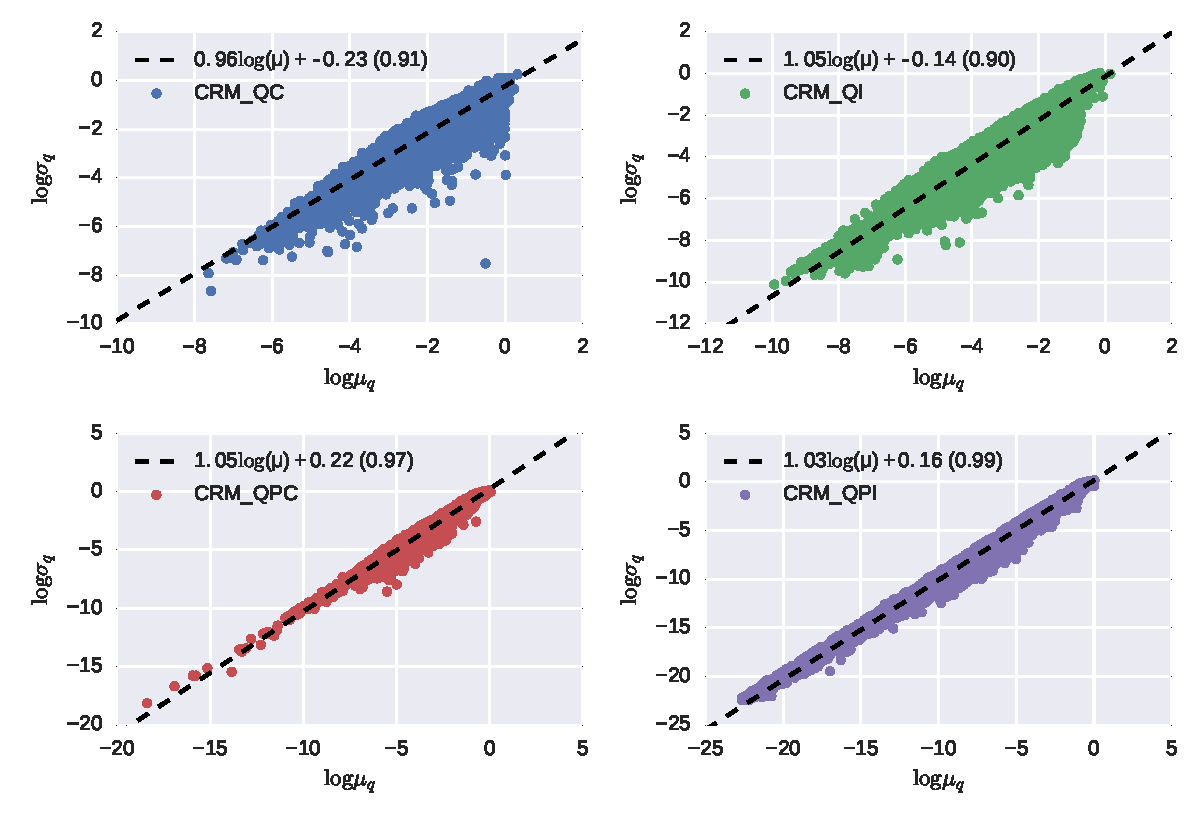
\includegraphics[width=\columnwidth]{graphics/condensate_std.pdf}
\caption{Scatter plots of condensate standard deviation against condensate mean for cloud liquid, cloud ice, precipitating liquid, and precipitating ice. Shown in the legend are the fit parameters to the relationship $\sigma = a \mu^b$, along with the coefficient of determination (r-squared) of the fit.}
\label{sgi_standard_deviation}
\end{figure}

Cloud physics parameterizations in large-scale (global) models diagnose the gridbox-mean cloud condensate amount, but most do not diagnose (or even implicitly assume) the gridbox-variance. In order to build a simple parameterization that can be used on typical GCM output, the gridbox-variance in total cloud and total precipitation condensate mixing ratio is represented here in terms of the gridbox-mean condensate. Figure \ref{sgi_standard_deviation} shows the standard deviation in cloud liquid (upper left), cloud ice (upper right), precipitating liquid (lower left) and precipitating ice (lower right) condensate mixing ratios versus gridbox mean cloud and precipitation condensate, respectively, again for a single day of SP-CAM output. Because the distribution of the mean and standard deviation of condensate mixing ratios is strongly skewed, these are shown on a log-log scale. The figure suggests that the standard deviation of condensate is strongly correlated with the mean, following an approximately linear relationship in log-log space. This suggests that the standard deviation $\sigma$ can be represented in terms of the mean $\mu$ for each condensate type by the functional relationship $\sigma = a \mu^b$, where $a$ and $b$ are constants that need to be parameterized. Note that taking the logarithm of both sides shows that this leads to a linear relationship in log-log space:
\begin{gather}
    \log \sigma = \log(a \mu^b) = \log a + b\log \mu
\end{gather}
Standard deviation is then fit to $\sigma = a \mu^b$ using non-linear least squares, and the results of the fit are indicated in each panel of Figure \ref{sgi_standard_deviation}. This provides a simple parameterization for condensate standard deviation, so that given just the gridbox mean values at each level, condensate standard deviation can be represented using this functional relationship. To generate stochastic subcolumns of clouds and precipitation using this, subcolumn cloud and precipitation occurrence flags are first generated using the framework described in Section \ref{subgrid2_generator_section}. Condensate amount is then generated for each hydrometeor type (cloud liquid, cloud ice, precipitating liquid, precipitating ice) using the framework described there, assuming that each hydrometeor type occupies \emph{all} of the cloudy or precipitating subcolumn elements, using the above parameterization to specify the standard deviation in terms of the mean. %By doing this, rather than diagnosing a total condensate and then partitioning, the condensate variance is reproduced separately for each hydrometeor type as faithfully as possible. This is important, because in general each hydrometeor type may have substantially different variance. Evidence for this is shown by Figure \ref{sgi_coefficient_of_variation}, which shows kernel density estimates (for the probability density function) of the coefficient of variability (normalized standard deviation) for each hydrometeor type. [is this really true? I think some tests I've done have shown this is not important. Regardless, maybe it makes more sense to separately reproduce each hydrometeor type...I can better reproduce the normalized condensate that way I think]

\begin{figure}
\centering
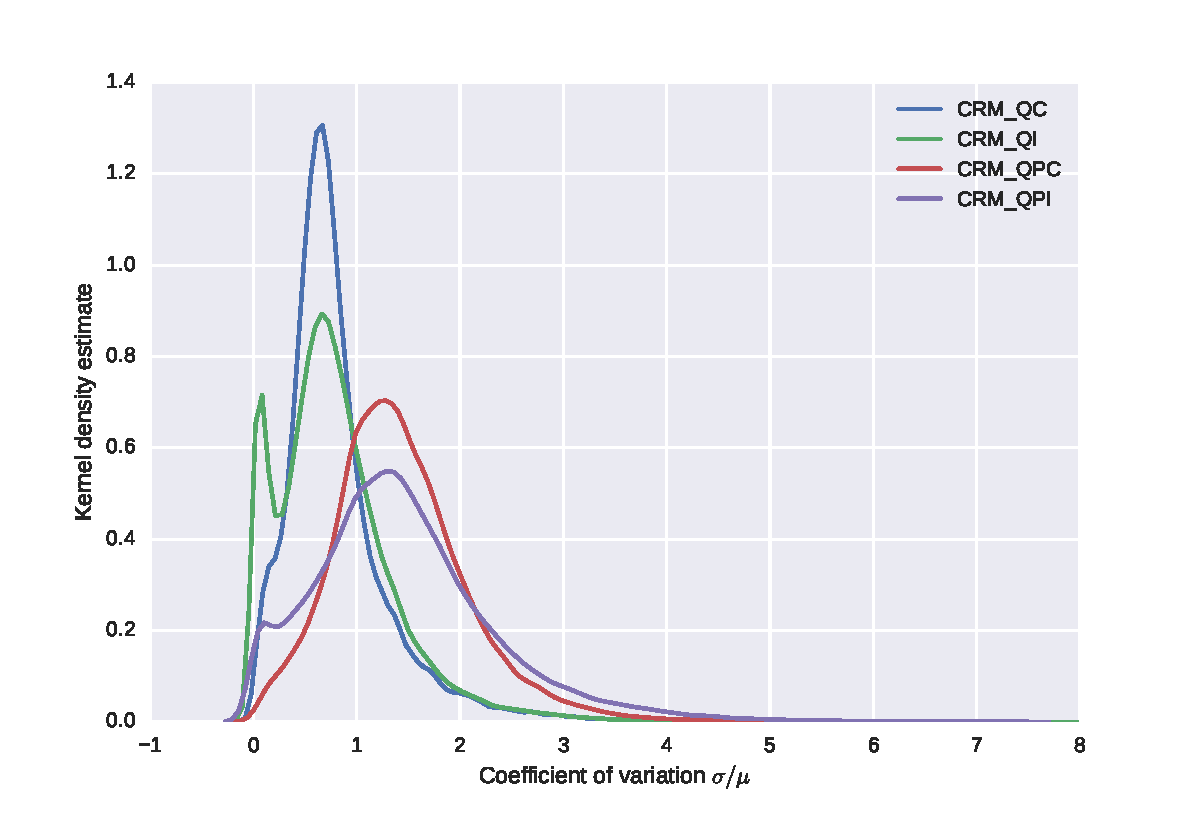
\includegraphics[width=\columnwidth]{graphics/coefficient_of_variation.pdf}
\caption{coefficient of variability}
\label{sgi_coefficient_of_variation}
\end{figure}

As discussed in the previous section in the context of the parameterization of overlap and rank correlation, these relationships are unlikely to hold under all conditions and cloud regimes, but this simple parameterization is sufficient for testing the sensitivity of simulated satellite cloud diagnostics to the treatment of unresolved variability. With overlap, rank correlation, and condensate distributions completely parameterized, an additional set of modified fields is created using the above described subcolumn generator, and referred to as ``GEN-VAR-PARAM''. In order to separately test the parameterization of overlap, rank correlation, and variability, another set of modified fields is created where the overlap, rank correlation, and gridbox variance is calculated at each gridbox directly from the CRM fields rather than parameterized. This case is referred to as ``GEN-VAR-CALC'' and represents the limit of performance that can be expected with this subcolumn generator. [NOTE: need to create this case...different from the GEN-VAR-CALC I created before, I want a case where overlap is calculated as well. New subcolumn generator (in Fortran 90) makes this even easier to do though]

The sensitivity test framework uses outputs from the SP-CAM to provide a plausible representation of cloud and precipitation structure and variability at scales similar to those at which the satellite retrievals are performed. While these outputs provide much higher resolution cloud fields than available in traditional GCMs, the fields simulated by the SP-CAM are in fact still model outputs, and may not perfectly simulate any observed cloud systems. Nonetheless, it has been shown here that the overlap and rank correlation statistics from SP-CAM are both qualitatively and quantitatively consistent with those found in observations from previous authors, and condensate variability is at least qualitatively consistent with previous studies as well, following similar statistical distributions. Thus, since the goal of this study is to evaluate the sensitivity of COSP diagnostics to these properties, rather than to develop a perfect parameterization of subgrid-scale overlap and variability, the SP-CAM output is sufficient for this purpose. %The task of parameterizing the overlap, rank correlation, and variance for inclusion in an actual large-scale model should involve a careful observational study, and should be consistent with assumptions made throughout the model. Such a task is left for future work, and will be discussed further at the end of the chapter.

In order to run the individual simulators directly on output from the SP-CAM, it is important that the fields simulated by the SP-CAM are on a scale similar to that at which the satellite retrievals are performed. The SP-CAM output used in this study was run using 4 km grid spacing for the embedded cloud-resolving model. MISR cloud top height retrievals are performed at a spatial scale of 1.1 km \citep{moroney_et_al_2002}, and the CloudSat cloud radar has a horizontal resolution of 1.4 km cross-track and 1.7 km along-track \citep{tanelli_et_al_2008}. While these scales are somewhat smaller than the 4 km grid used by the SP-CAM CRM, the differences are small and are unlikely to affect the results of the sensitivity study performed with the 4 km fields.

\section{Quantifying improvements in COSP-simulated diagnostics}
\label{subgrid2_results_section}
[!!! TODO: write section !!!]
With the improved subcolumn generator described in the preceeding sections, the sensitivity of the COSP diagnostics to the improvements can be quantified using the same framework used in the previous chapter to quantify the sensitivities to overlap and homogeneous condensate assumptions. Again, a series of modified cloud and precipitation condensate fields are created from a month-long SP-CAM simulation. COSP is then run on each set of modified fields, and the COSP outputs are compared with one another to quantify the sensitivity to different aspects of the improved subcolumn generator. These cases are described below.

\begin{figure}
\centering
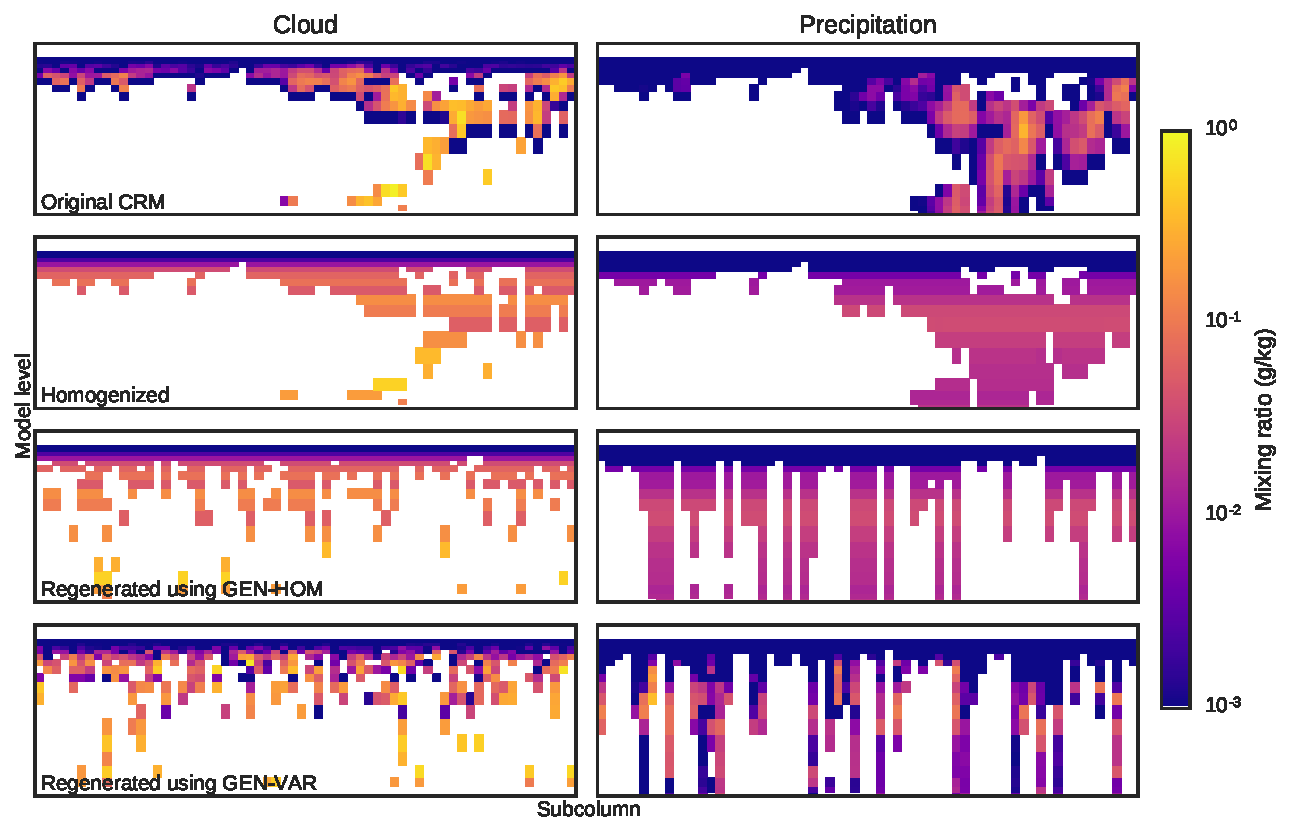
\includegraphics[width=\columnwidth]{graphics/mxratio_gen-var.pdf}
\caption{Cases with improved subcolumn generator following R04.}
\label{mxratio_gen-var}
\end{figure}

The first two cases are identical to those used in the previous chapter. The first case is the baseline case, created by running COSP on the original, unmodified CRM fields from the SP-CAM simulation. The second case is the homogenized case (CRM-HOM), created by replacing the cloud and precipitation condensate with the gridbox-means (by level), everywhere where cloud and precipitation exist in the original CRM fields. The remaining cases are generated by, again, first calculating the gridbox-mean profiles of cloud fraction, precipitation fraction, and cloud and precipitation condensate from the original CRM fields, and then using various iterations of the subcolumn generator to regenerate subcolumn condensate fields from the gridbox-mean profiles. The first of these uses the generalized overlap scheme described above, but with \emph{homogeneous} cloud and precipitation condensate (GEN-HOM). The second uses the full subcolumn generator described above with generalized overlap and variable condensate (GEN-VAR).

As in the previous chapter, the sensitivity to both the overlap and the variability treatment can be quantified by taking appropriate differences between the outputs from these different cases. The only difference between the CRM-HOM and GEN-HOM cases is the treatment of cloud (and precipitation) overlap, so the difference between the outputs from these cases quantifies the component of the error due to the generalized overlap treatment alone. The component of the error due to the treatment of variability is quantified by calculating the residual between the total error in using the full subcolumn generator (GEN-VAR minus CRM) and the component of the error due to the treatment of overlap (GEN-HOM minus CRM-HOM). The total error $E_{\rm total}$ and the overlap and variability components $E_{\rm overlap}$ and $E_{\rm variability}$ are calculated for a simulated satellite diagnostic quantity $X$ then as
\begin{gather}
E_{\rm total} = X_{\rm GEN-VAR} - X_{\rm CRM} \\
E_{\rm overlap} = X_{\rm GEN-HOM} - X_{\rm CRM-HOM} \\
E_{\rm variability} = (X_{\rm GEN-VAR} - X_{\rm CRM}) - (X_{\rm GEN-HOM} - X_{\rm CRM-HOM})
\end{gather}

%Likewise, the main difference between the GEN-HOM and GEN-VAR cases is the treatment of variability, so calculating the difference between the outputs from these cases quantifies the component of the error due to the treatment of variability alone. [TODO: check that this is right...slightly different than how I did this before...]

\section{Reduced errors in simulated passive remote sensing diagnostics}
\label{subgrid2_passive_section}
\begin{figure}
\centering
\caption{Errors in MISR-simulated cloud area by cloud top height arising due to using the improved GEN-VAR subcolumn generator to regenerate subcolumns from gridbox-mean profiles (left), the component of the error due to the treatment of variability (middle), and the component of the error due to the treatment of overlap (right).}
\label{sgi_cldmisr_maps_diff}
\end{figure}
Figure \ref{sgi_cldmisr_maps_diff} shows the errors in MISR-simulated cloud area by cloud top height that arise due to using the new GEN-VAR subcolumn generator to regenerate subcolumn cloud and precipitation condensate fields from gridbox-mean profiles, in the same manner in which Figure \ref{sg_cldmisr_maps_diff} shows errors that arise due to using SCOPS/PREC\_SCOPS with maximum-random overlap and homogeneous condensate (MRO-HOM). Comparing Figures \ref{sgi_cldmisr_maps_diff} and \ref{sg_cldmisr_maps_diff} it is clear that the GEN-VAR scheme has substantially reduced the errors identified in chapter \ref{sg_chapter} due to both the treatment of variability and overlap. Errors due to the treatment of variability are everywhere less than ?? using the new scheme, compared with errors are large as ?? using homogeneous condensate. Errors due to the overlap treatment are similarly reduced, from regional errors as large as 10\% using MRO down to ?? using the GEN-VAR scheme. The total error that arises due to regenerating subcolumns using the subcolumn generator has likewise been reduced, but more importantly the compensating errors between high and low-topped clouds have been nearly eliminated using the new scheme. Similar reductions in errors are demonstrated for ISCCP and MODIS-simulated cloud area by cloud top height, shown in Figures \ref{sgi_cldisccp_maps_diff} and \ref{sgi_cldmodis_maps_diff}

\begin{figure}
\centering
\caption{Errors in ISCCP-simulated cloud area by cloud top pressure.}
\label{sgi_cldisccp_maps_diff}
\end{figure}

\begin{figure}
\centering
\caption{Errors in MODIS-simulated cloud area by cloud top pressure.}
\label{sgi_cldmodis_maps_diff}
\end{figure}

Regional errors in both cloud top height and cloud optical depth are also reduced using the new scheme, as shown in Figures ??. [TODO: discussion of CTH-OD differences; compare with previous chapter, also on the TODO list]


\section{Reduced errors in simulated CloudSat reflectivity and hydrometeor occurrence}
\label{subgrid2_active_section}
\begin{figure}
\centering
\caption{Errors in CloudSat-simulated hydrometeor occurrence ($Z_e > -27.5$ dBZ) arising due to using GEN-VAR to regenerate subcolumns of cloud and precipitation (top), as well as components due to both the VAR treatment of variability (middle) and the GEN treatment of overlap (bottom).}
\label{sgi_hfba_zonal_diff}
\end{figure}
Figure \ref{sgi_hfba_zonal_diff} shows the errors in the zonally-averaged CloudSat-simulated hydrometeor occurrence fraction. Comparing these errors to those shown in Figure \ref{sg_hfba_zonal_diff} again shows a substantial reduction in errors of all types using the improved subcolumn generator relative to those errors that result from using SCOPS/PREC\_SCOPS. Maximum errors have been reduced from ?? to ?? using the improved scheme. [More here, remaining errors? Where are the errors?]. This represents a reduction of the relative error from ?? down to ??; a marked improvement [more here].

\begin{figure}
\centering
\caption{Errors in CloudSat-simulated reflectivity with height histograms for the NH Tropics (0 to 10 degrees north).}
\label{sgi_cfadDbze94_nhtropics_diff}
\end{figure}
Figure \ref{sgi_cfadDbze94_nhtropics_diff} shows errors in CloudSat-simulated reflectivity with height histograms for the Northern Hemisphere Tropics. The figure shows again a reduction in errors of all types from using the GEN-VAR scheme to regenerate subcolumns. The largest impact is the inclusion of heterogeneous condensate, as after adjusting for precipitation, the homogeneous errors dominated the errors using MRO-HOM scheme shown in the previous chapter. 

[What else to say here? Further discussion of values of both absolute and relative errors; quantify reduction of errors, i.e., ``this is a 20\% reduction in error from the MRO-HOM to the GEN-VAR'']

\section{Discussion}
\label{subgrid2_discussion_section}
[!!! TODO: write this entire section !!!]
Of course, it has been recognized that subgrid-scale variability, including cloud and precipitation occurrence overlap and condensate amount, effect many important processes in large-scale models, and some researchers are trying to develop explicit subgrid treatments for GCMS. This includes so-called ``statistical'' or ``assumed probability distribution'' schemes, which predict the evolution of not only the mean, but also the probability distribution of total water (and hence the cloud and precipitation condensate) within each grid-box \citep[e.g.,][]{tompkins_2002}. There has been growing interest in using these schemes in GCMs. One such example of this is the Cloud Layers Unified By Binormals \citep[CLUBB;][]{golaz_et_al_2002} scheme, which is being implemented into the NCAR CAM (A. Gettelman, personal communication). Because these schemes explicitly assume a probability distribution for the subgrid variability of condensate, they are a natural fit to the stochastic treatment of subgrid clouds and precipitation used in COSP to simulate satellite retrievals (and also to radiation schemes that use stochastic treatments of subgrid clouds such as the McICA \citep{pincus_et_al_2003}, because the same distribution of condensate can be shared between these different components of the model. As shown here for simulated satellite diagnostics and by others for calculated radiative fluxes, these assumptions can have a large impact on diagnosed cloud effects, and thus consistency between cloud treatments in the different parts of the model is necessary in order to obtain a consistent picture of the performance of models in simulating clouds.

%% END OF CHAPTER
